\section{Requirements}
\label{sec:requirements}
Zur \gls{Spezifikation} der Smartwatch wurden - neben den in Abschnitt~\ref{sec:use_cases} beschriebenen \glspl{Use-Case} - die wichtigsten \glspl{Requirement} gesammelt und festgehalten. Um die Übersicht und Nachvollziehbarkeit zu verbessern, werden diese in die folgenden Kategorien eingeteilt:

\begin{itemize}
	\item Ausgabe -- Ausgabe beinhaltet alle Requirements, die sich auf die grafische und auf die akustische Ausgabe beziehen.
	\item \gls{Usability} -- Alle Requirements zur Beschreibung der Bedienbarkeit der Smartwatch
	\item Kapazität -- Alle Requirements bezüglich der Energieversorgung
	\item Funktionen -- Funktionen beinhaltet alle \glspl{Requirement}, die konkrete Funktionen der Smartwatch beschreiben
	\item \gls{Ergonomie} -- Ergonomische \glspl{Requirement} beschreiben das Design und die physische Eigenschaften der Smartwatch.
\end{itemize}

Das Package-Diagram in Abbildung~\ref{fig:package_diagram_requirements} teilt die \glspl{Requirement}-Kategorien in einzelne \glspl{Package} auf.

\begin{figure}
\centering\
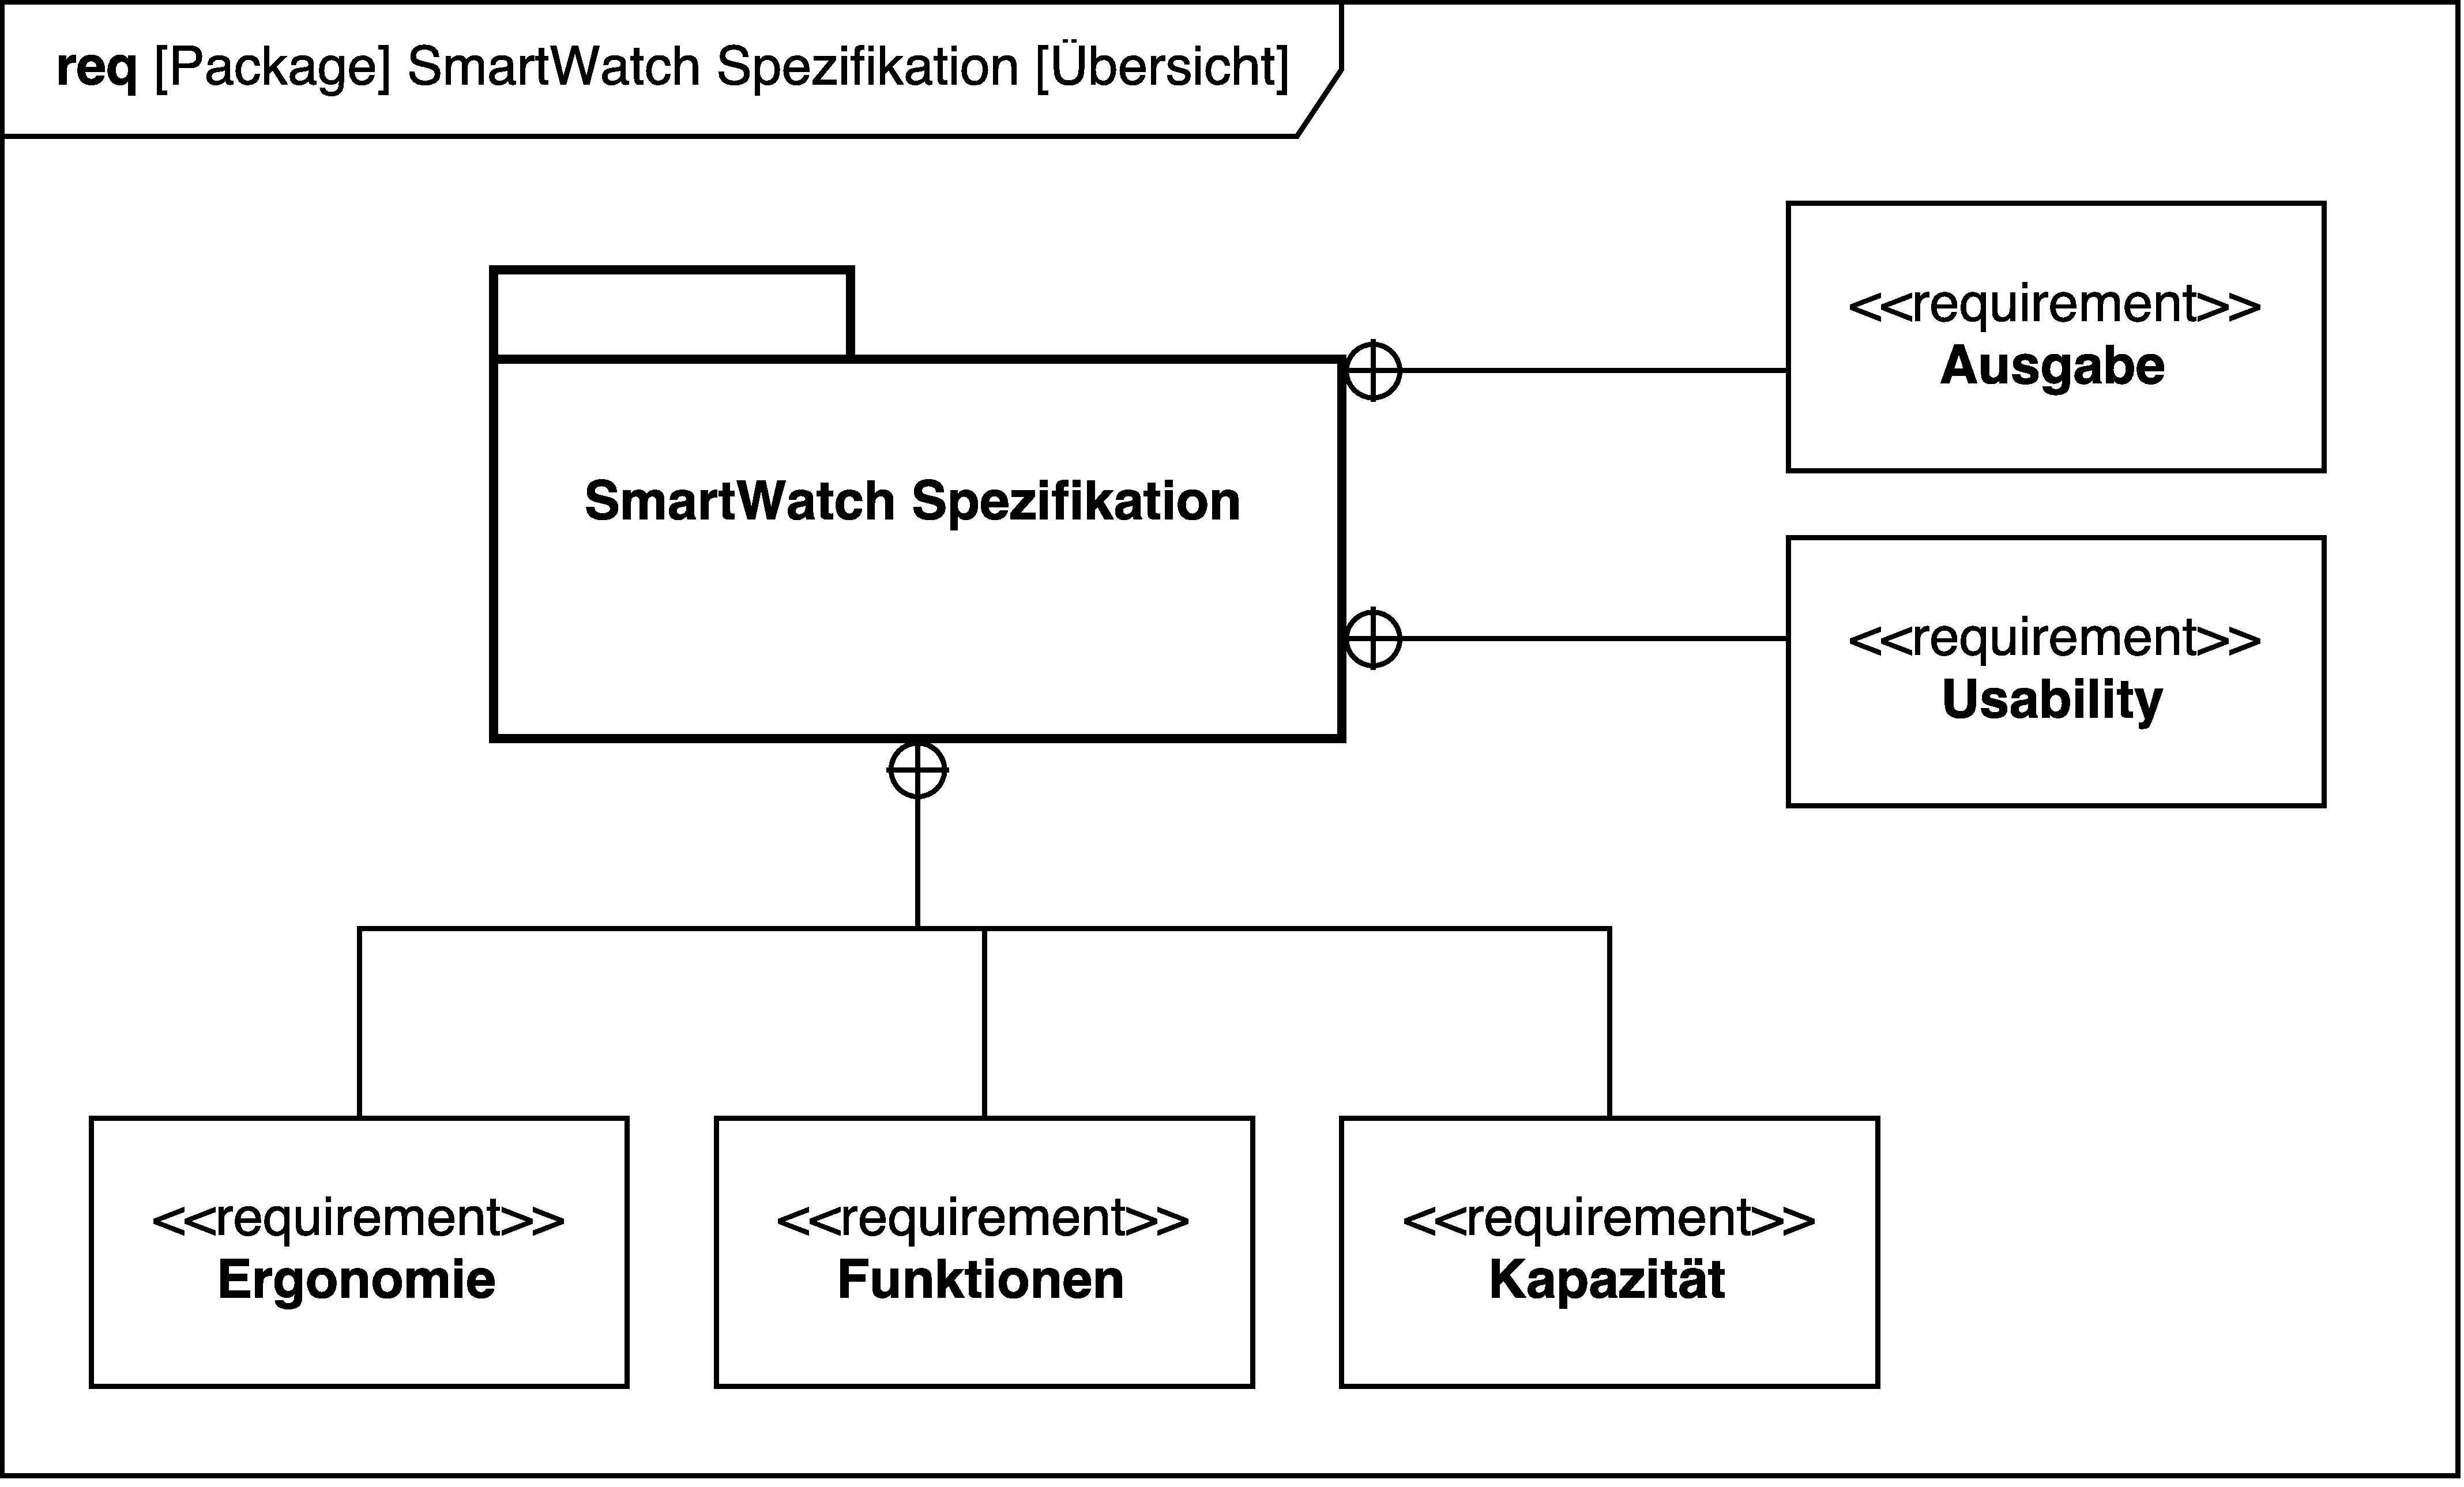
\includegraphics[width=14cm]{img/package_diagram_smartWatch_requirements}
\caption[Requirements: Package Diagram]{Package Diagram der einzelnen Requirement-Kategorien}
\label{fig:package_diagram_requirements}
\end{figure}

Tabelle~\ref{tab:table_requirements} enthält die gesammelten Requirements aufgeteilt in die einzelnen Kategorien.

Abbildung~\ref{fig:requirement_diagram_akku} zeigt das Requirement Diagram der Requirements der Kategorie Kapazität. Besonders hervorzuheben ist die Abhängigkeit zwischen \textit{Akkuladezeit} und \textit{Akku: Induktionsladen}. Mittels des \gls{Stereotyp} \textit{deriveReqt} wird signalisiert, dass \textit{Akku: Induktionsladen} eine Erweiterung des Requirements \textit{Akkuladezeit} ist, das bedeutet, dass für das Laden mittels Induktion die Ladezeitvorgabe (2 Stunden) des Akkuladezeit-Requirements gilt.

\begin{figure}
\centering\
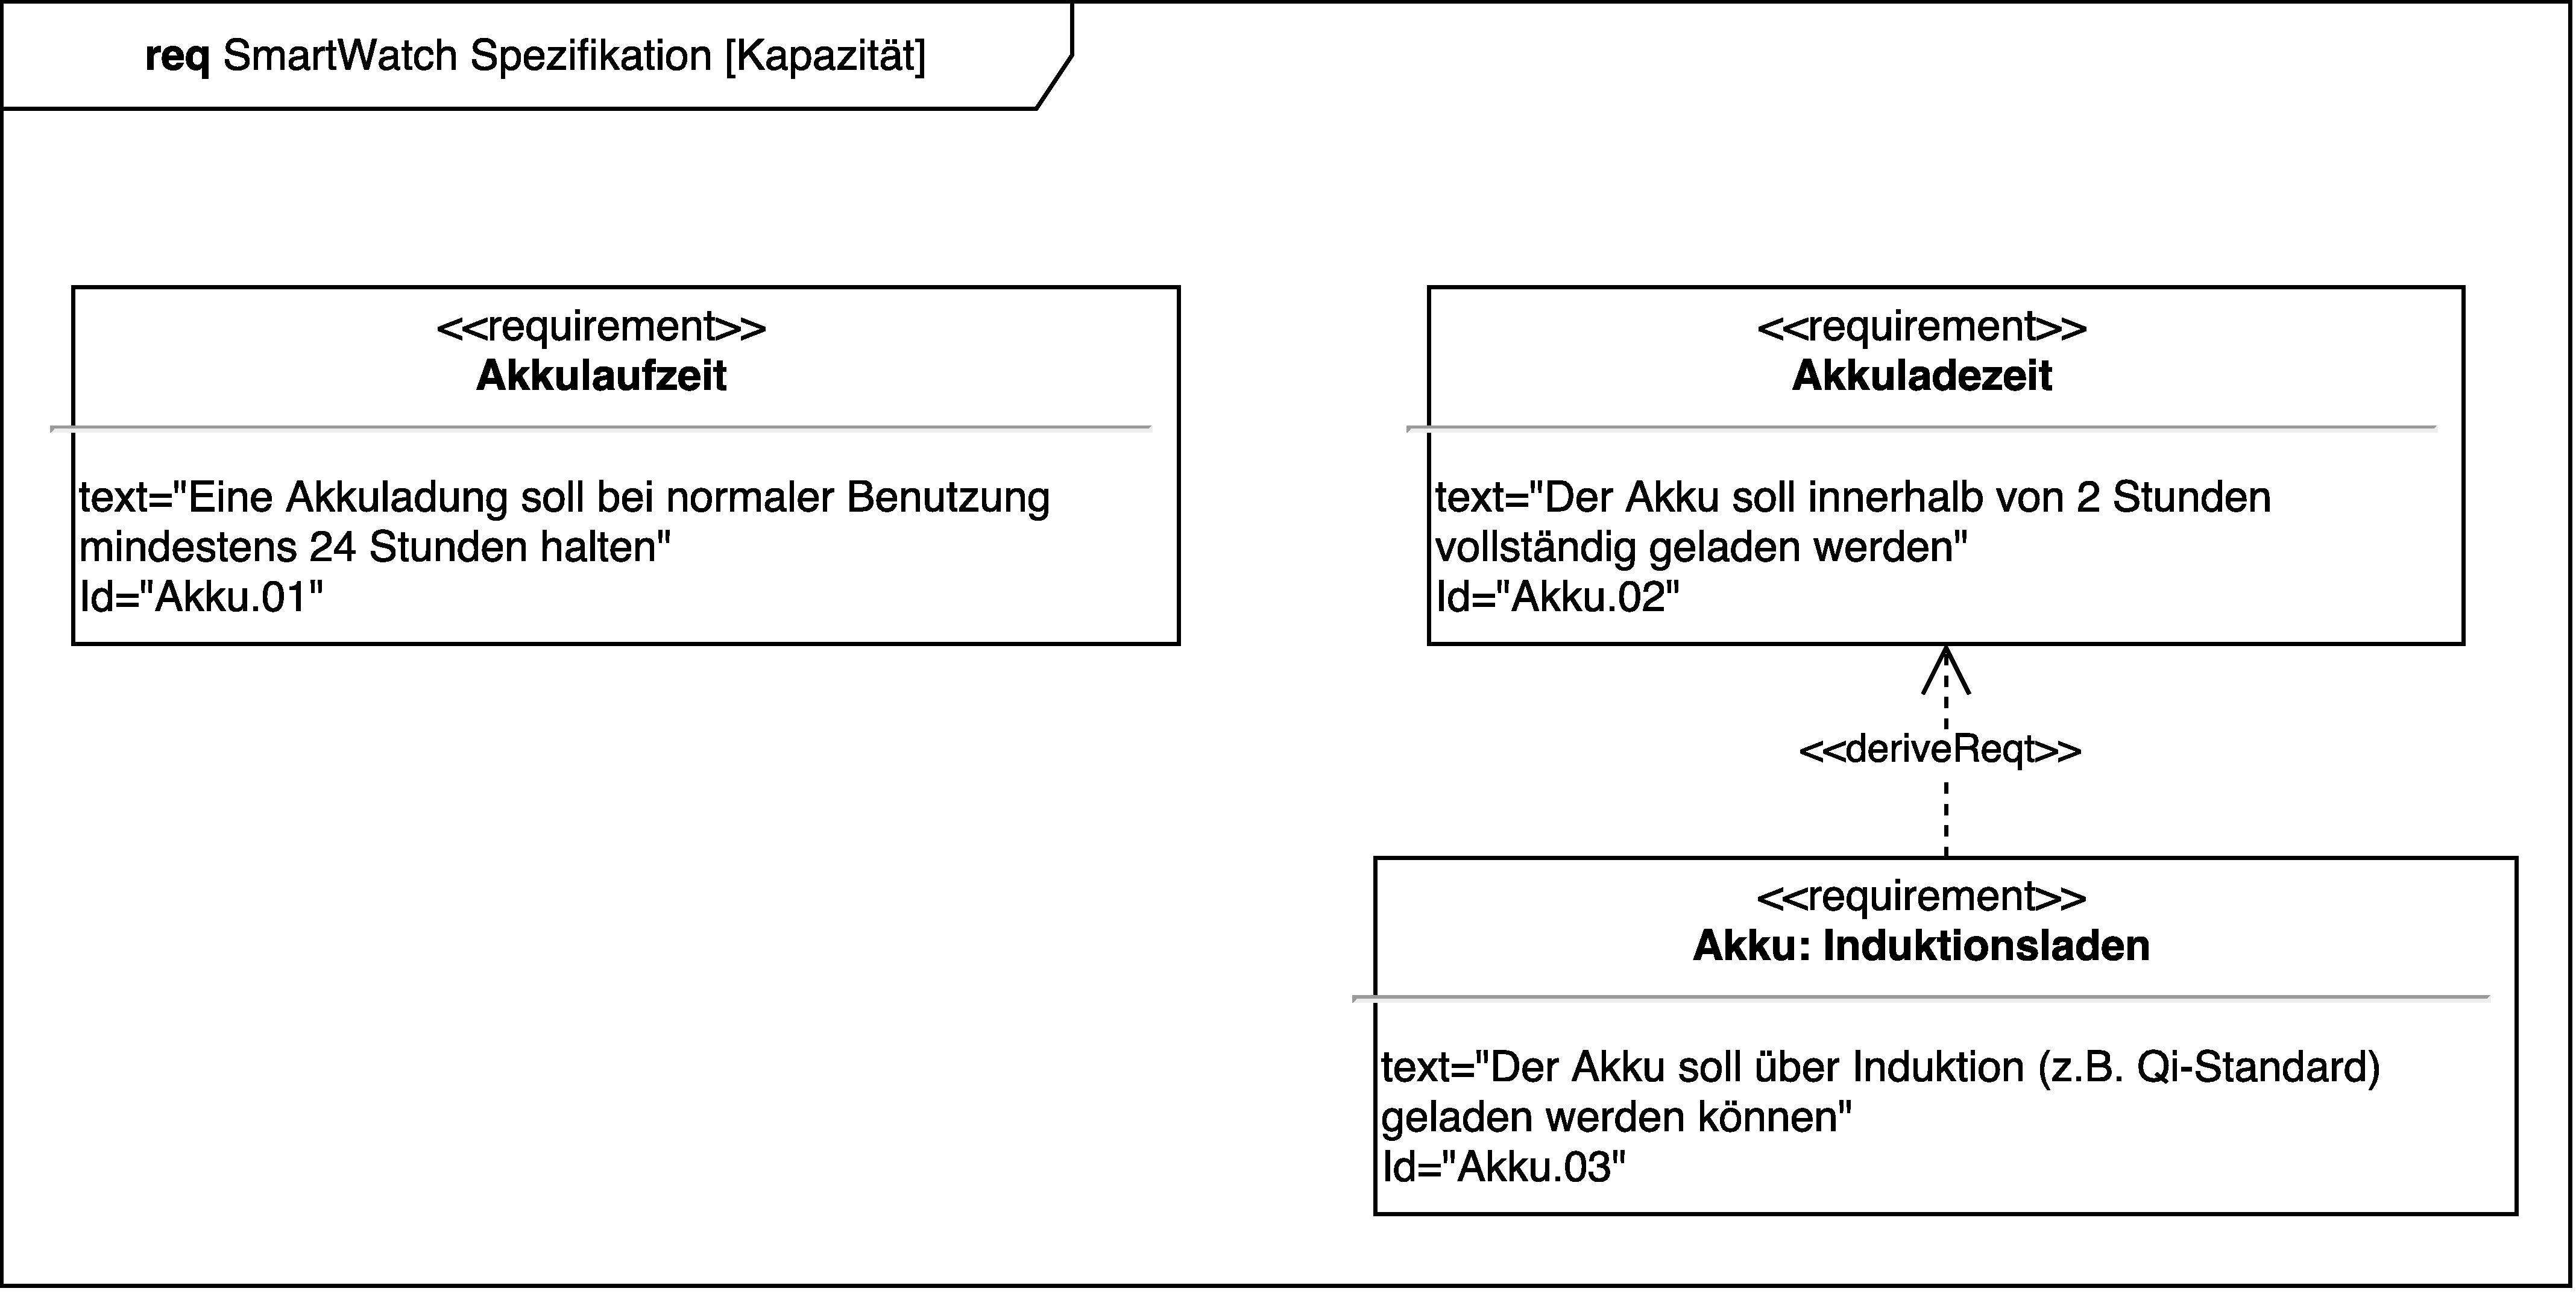
\includegraphics[width=14cm]{img/requirement_diagram_akku}
\caption[Requirements: Kapazität]{Requirement Diagram der Requirements der Kategorie Kapazität}
\label{fig:requirement_diagram_akku}
\end{figure}
